\begin{enumerate}[label=\thesection.\arabic*,ref=\thesection.\theenumi]
\numberwithin{equation}{enumi}
\numberwithin{figure}{enumi}
\numberwithin{table}{enumi}
\item Prove that the line of centres of two intersecting circles subtends equal angles at the two points of intersection.
\\
    \solution 
\label{chapters/9/10/6/1}
\iffalse
\documentclass[12pt]{article}
\usepackage{graphicx}
\usepackage{amsmath}
\usepackage{mathtools}
\usepackage{gensymb}
\usepackage{amssymb}
\usepackage{tikz}
\usetikzlibrary{arrows,shapes,automata,petri,positioning,calc}
\usepackage{hyperref}
\usepackage{tikz}
\usetikzlibrary{matrix,calc}
\usepackage[margin=0.5in]{geometry}

\providecommand{\norm}[1]{\left\lVert#1\right\rVert}
\newcommand{\myvec}[1]{\ensuremath{\begin{pmatrix}#1\end{pmatrix}}}
\let\vec\mathbf
%\providecommand $${\norm}[1]{\left\lVert#1\right\rVert}$$
\providecommand{\abs}[1]{\left\vert#1\right\vert}
\let\vec\mathbf

\newcommand{\mydet}[1]{\ensuremath{\begin{vmatrix}#1\end{vmatrix}}}
\providecommand{\brak}[1]{\ensuremath{\left(#1\right)}}
\providecommand{\lbrak}[1]{\ensuremath{\left(#1\right.}}
\providecommand{\rbrak}[1]{\ensuremath{\left.#1\right)}}
\providecommand{\sbrak}[1]{\ensuremath{{}\left[#1\right]}}

\providecommand{\brak}[1]{\ensuremath{\left(#1\right)}}
\providecommand{\norm}[1]{\left\lVert#1\right\rVert}
\newcommand{\solution}{\noindent \textbf{Solution: }}

\let\vec\mathbf
\def\inputGnumericTable{}
\usepackage{color}                                            %%
    \usepackage{array}                                            %%
    \usepackage{longtable}                                        %%
    \usepackage{calc}                                             %%
    \usepackage{multirow}                                         %%
    \usepackage{hhline}                                           %%
    \usepackage{ifthen}
\usepackage{array}
\usepackage{amsmath}   % for having text in math mode
\usepackage{listings}
\lstset{
language=tex,
frame=single, 
breaklines=true
}
\newenvironment{Figure}
  {\par\medskip\noindent\minipage{\linewidth}}
  {\endminipage\par\medskip}
\begin{document}
\begin{center}
\textbf\large{CLASS-9\\CHAPTER-10 \\ CIRCLES}

\end{center}
\section*{Excercise 10.6}

\section*{\large Solution}:
\fi
The input parameters are available in Table 
	\ref{tab:chapters/9/10/6/1/table1}.
\begin{figure}[h!]
\centering
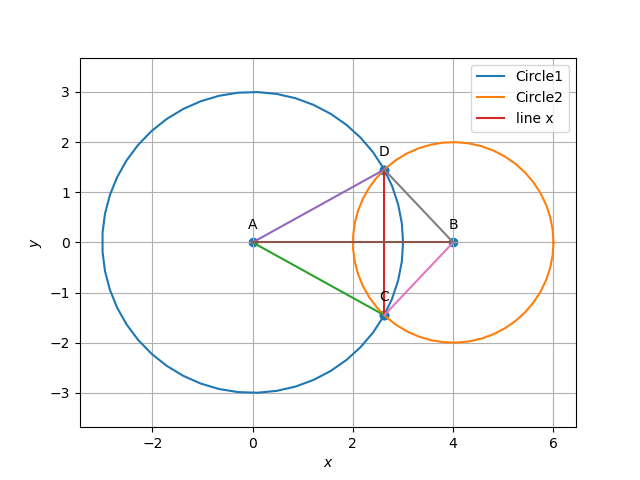
\includegraphics[width=\columnwidth]{chapters/9/10/6/1/figs/circle3.png}
\caption{}
\label{fig:chapters/9/10/6/1/Fig1}
\end{figure}



\begin{table}[h!]
	\small
	\centering
	%\subimport{../chapters/9/10/6/1/tables/}{table1.tex}
     %%%%%%%%%%%%%%%%%%%%%%%%%%%%%%%%%%%%%%%%%%%%%%%%%%%%%%%%%%%%%%%%%%%%%%
%%                                                                  %%
%%  This is the header of a LaTeX2e file exported from Gnumeric.    %%
%%                                                                  %%
%%  This file can be compiled as it stands or included in another   %%
%%  LaTeX document. The table is based on the longtable package so  %%
%%  the longtable options (headers, footers...) can be set in the   %%
%%  preamble section below (see PRAMBLE).                           %%
%%                                                                  %%
%%  To include the file in another, the following two lines must be %%
%%  in the including file:                                          %%
%%        \def\inputGnumericTable{}                                 %%
%%  at the beginning of the file and:                               %%
%%        \input{name-of-this-file.tex}                             %%
%%  where the table is to be placed. Note also that the including   %%
%%  file must use the following packages for the table to be        %%
%%  rendered correctly:                                             %%
%%    \usepackage[latin1]{inputenc}                                 %%
%%    \usepackage{color}                                            %%
%%    \usepackage{array}                                            %%
%%    \usepackage{longtable}                                        %%
%%    \usepackage{calc}                                             %%
%%    \usepackage{multirow}                                         %%
%%    \usepackage{hhline}                                           %%
%%    \usepackage{ifthen}                                           %%
%%  optionally (for landscape tables embedded in another document): %%
%%    \usepackage{lscape}                                           %%
%%                                                                  %%
%%%%%%%%%%%%%%%%%%%%%%%%%%%%%%%%%%%%%%%%%%%%%%%%%%%%%%%%%%%%%%%%%%%%%



%%  This section checks if we are begin input into another file or  %%
%%  the file will be compiled alone. First use a macro taken from   %%
%%  the TeXbook ex 7.7 (suggestion of Han-Wen Nienhuys).            %%
\def\ifundefined#1{\expandafter\ifx\csname#1\endcsname\relax}


%%  Check for the \def token for inputed files. If it is not        %%
%%  defined, the file will be processed as a standalone and the     %%
%%  preamble will be used.                                          %%
\ifundefined{inputGnumericTable}

%%  We must be able to close or not the document at the end.        %%
	\def\gnumericTableEnd{\end{document}}


%%%%%%%%%%%%%%%%%%%%%%%%%%%%%%%%%%%%%%%%%%%%%%%%%%%%%%%%%%%%%%%%%%%%%%
%%                                                                  %%
%%  This is the PREAMBLE. Change these values to get the right      %%
%%  paper size and other niceties.                                  %%
%%                                                                  %%
%%%%%%%%%%%%%%%%%%%%%%%%%%%%%%%%%%%%%%%%%%%%%%%%%%%%%%%%%%%%%%%%%%%%%%

	\documentclass[12pt%
			  %,landscape%
                    ]{report}
       \usepackage[latin1]{inputenc}
       \usepackage{fullpage}
       \usepackage{color}
       \usepackage{array}
       \usepackage{longtable}
       \usepackage{calc}
       \usepackage{multirow}
       \usepackage{hhline}
       \usepackage{ifthen}
       \usepackage{gensymb}
       \usepackage{graphicx}
\usepackage{amsmath}
\usepackage{mathtools}
\newcommand{\mydet}[1]{\ensuremath{\begin{vmatrix}#1\end{vmatrix}}}
\providecommand{\brak}[1]{\ensuremath{\left(#1\right)}}
\providecommand{\norm}[1]{\left\lVert#1\right\rVert}
\newcommand{\solution}{\noindent \textbf{Solution: }}
\newcommand{\myvec}[1]{\ensuremath{\begin{pmatrix}#1\end{pmatrix}}}
\let\vec\mathbf
	\begin{document}


%%  End of the preamble for the standalone. The next section is for %%
%%  documents which are included into other LaTeX2e files.          %%
\else

%%  We are not a stand alone document. For a regular able, we will %%
%%  have no preamble and only define the closing to mean nothing.   %%
    \def\gnumericTableEnd{}

%%  If we want landscape mode in an embedded document, comment out  %%
%%  the line above and uncomment the two below. The table will      %%
%%  begin on a new page and run in landscape mode.                  %%
%       \def\gnumericTableEnd{\end{landscape}}
%       \begin{landscape}


%%  End of the else clause for this file being \input.              %%
\fi

%%%%%%%%%%%%%%%%%%%%%%%%%%%%%%%%%%%%%%%%%%%%%%%%%%%%%%%%%%%%%%%%%%%%%%
%%                                                                  %%
%%  The rest is the gnumeric table, except for the closing          %%
%%  statement. Changes below will alter the table's appearance.     %%
%%                                                                  %%
%%%%%%%%%%%%%%%%%%%%%%%%%%%%%%%%%%%%%%%%%%%%%%%%%%%%%%%%%%%%%%%%%%%%%%
\providecommand{\gnumericmathit}[1]{#1} 
%%  Uncomment the next line if you would like your numbers to be in %%
%%  italics if they are italizised in the gnumeric table.           %%
%\renewcommand{\gnumericmathit}[1]{\mathit{#1}}
\providecommand{\gnumericPB}[1]%
{\let\gnumericTemp=\\#1\let\\=\gnumericTemp\hspace{0pt}}
 \ifundefined{gnumericTableWidthDefined}
        \newlength{\gnumericTableWidth}
        \newlength{\gnumericTableWidthComplete}
        \newlength{\gnumericMultiRowLength}
        \global\def\gnumericTableWidthDefined{}
 \fi
%% The following setting protects this code from babel shorthands.  %%
 \ifthenelse{\isundefined{\languageshorthands}}{}{\languageshorthands{english}}
%%  The default table format retains the relative column widths of  %%
%%  gnumeric. They can easily be changed to c, r or l. In that case %%
%%  you may want to comment out the next line and uncomment the one %%
%%  thereafter                                                      %%
\providecommand\gnumbox{\makebox[0pt]}
%%\providecommand\gnumbox[1][]{\makebox}

%% to adjust positions in multirow situations                       %%
\setlength{\bigstrutjot}{\jot}
\setlength{\extrarowheight}{\doublerulesep}

%%  The \setlongtables command keeps column widths the same across  %%
%%  pages. Simply comment out next line for varying column widths.  %%
\setlongtables

\setlength\gnumericTableWidth{%
	40pt+%
	35pt+%
	210pt+%
0pt}
\def\gumericNumCols{3}
\setlength\gnumericTableWidthComplete{\gnumericTableWidth+%
         \tabcolsep*\gumericNumCols*2+\arrayrulewidth*\gumericNumCols}
\ifthenelse{\lengthtest{\gnumericTableWidthComplete > \linewidth}}%
         {\def\gnumericScale{\ratio{\linewidth-%
                        \tabcolsep*\gumericNumCols*2-%
                        \arrayrulewidth*\gumericNumCols}%
{\gnumericTableWidth}}}%
{\def\gnumericScale{1}}

%%%%%%%%%%%%%%%%%%%%%%%%%%%%%%%%%%%%%%%%%%%%%%%%%%%%%%%%%%%%%%%%%%%%%%
%%                                                                  %%
%% The following are the widths of the various columns. We are      %%
%% defining them here because then they are easier to change.       %%
%% Depending on the cell formats we may use them more than once.    %%
%%                                                                  %%
%%%%%%%%%%%%%%%%%%%%%%%%%%%%%%%%%%%%%%%%%%%%%%%%%%%%%%%%%%%%%%%%%%%%%%

\ifthenelse{\isundefined{\gnumericColA}}{\newlength{\gnumericColA}}{}\settowidth{\gnumericColA}{\begin{tabular}{@{}p{40pt*\gnumericScale}@{}}x\end{tabular}}
\ifthenelse{\isundefined{\gnumericColB}}{\newlength{\gnumericColB}}{}\settowidth{\gnumericColB}{\begin{tabular}{@{}p{35pt*\gnumericScale}@{}}x\end{tabular}}
\ifthenelse{\isundefined{\gnumericColC}}{\newlength{\gnumericColC}}{}\settowidth{\gnumericColC}{\begin{tabular}{@{}p{210pt*\gnumericScale}@{}}x\end{tabular}}

\begin{longtable}[c]{%
	b{\gnumericColA}%
	b{\gnumericColB}%
	b{\gnumericColC}%
	}

%%%%%%%%%%%%%%%%%%%%%%%%%%%%%%%%%%%%%%%%%%%%%%%%%%%%%%%%%%%%%%%%%%%%%%
%%  The longtable options. (Caption, headers... see Goosens, p.124) %%
%	\caption{The Table Caption.}             \\	%
% \hline	% Across the top of the table.
%%  The rest of these options are table rows which are placed on    %%
%%  the first, last or every page. Use \multicolumn if you want.    %%

%%  Header for the first page.                                      %%
%	\multicolumn{3}{c}{The First Header} \\ \hline 
%	\multicolumn{1}{c}{colTag}	%Column 1
%	&\multicolumn{1}{c}{colTag}	%Column 2
%	&\multicolumn{1}{c}{colTag}	\\ \hline %Last column
%	\endfirsthead

%%  The running header definition.                                  %%
%	\hline
%	\multicolumn{3}{l}{\ldots\small\slshape continued} \\ \hline
%	\multicolumn{1}{c}{colTag}	%Column 1
%	&\multicolumn{1}{c}{colTag}	%Column 2
%	&\multicolumn{1}{c}{colTag}	\\ \hline %Last column
%	\endhead

%%  The running footer definition.                                  %%
%	\hline
%	\multicolumn{3}{r}{\small\slshape continued\ldots} \\
%	\endfoot

%%  The ending footer definition.                                   %%
%	\multicolumn{3}{c}{That's all folks} \\ \hline 
%	\endlastfoot
%%%%%%%%%%%%%%%%%%%%%%%%%%%%%%%%%%%%%%%%%%%%%%%%%%%%%%%%%%%%%%%%%%%%%%

\hhline{|-|-|-}
	 \multicolumn{1}{|p{\gnumericColA}|}%
	{\gnumericPB{\raggedright}\gnumbox[l]{\textbf{Symbol}}}
	&\multicolumn{1}{p{\gnumericColB}|}%
	{\gnumericPB{\raggedright}\gnumbox[l]{\textbf{Values}}}
	&\multicolumn{1}{p{\gnumericColC}|}%
	{\gnumericPB{\raggedright}\gnumbox[l]{\textbf{Description}}}
\\
\hhline{|---|}
	 \multicolumn{1}{|p{\gnumericColA}|}%
	{\gnumericPB{\raggedright}\gnumbox[l]{$\vec{A}$}}
	&\multicolumn{1}{p{\gnumericColB}|}%
	{\gnumericPB{\raggedright}\gnumbox[l]{\myvec{0\\0}}}
	&\multicolumn{1}{p{\gnumericColC}|}%
	{\gnumericPB{\raggedright}\gnumbox[l]{Center of circle 1}}
\\
\hhline{|---|}
	 \multicolumn{1}{|p{\gnumericColA}|}%
	{\gnumericPB{\raggedright}\gnumbox[l]{$r_1$}}
	&\multicolumn{1}{p{\gnumericColB}|}%
	{\gnumericPB{\raggedright}\gnumbox[l]{3 units}}
	&\multicolumn{1}{p{\gnumericColC}|}%
	{\gnumericPB{\raggedright}\gnumbox[l]{Radius of the circle 1 }}
\\
\hhline{|---|}
	 \multicolumn{1}{|p{\gnumericColA}|}%
	{\gnumericPB{\raggedright}\gnumbox[l]{$\vec{B}$}}
	&\multicolumn{1}{p{\gnumericColB}|}%
	{\gnumericPB{\raggedright}\gnumbox[l]{\myvec{4\\0}}}
	&\multicolumn{1}{p{\gnumericColC}|}%
	{\gnumericPB{\raggedright}\gnumbox[l]{Center of circle 2}}
\\
\hhline{|---|}
	 \multicolumn{1}{|p{\gnumericColA}|}%
	{\gnumericPB{\raggedright}\gnumbox[l]{$r_2$}}
	&\multicolumn{1}{p{\gnumericColB}|}%
	{\gnumericPB{\raggedright}\gnumbox[l]{2 units}}
	&\multicolumn{1}{p{\gnumericColC}|}%
	{\gnumericPB{\raggedright}\gnumbox[l]{Radius of circle 2}}
\\
\hhline{|---|}
	 \multicolumn{1}{|p{\gnumericColA}|}%
	{\gnumericPB{\raggedright}\gnumbox[l]{$\vec{e}_1$}}
	&\multicolumn{1}{p{\gnumericColB}|}%
	{\gnumericPB{\raggedright}\gnumbox[l]{\myvec{1\\0}}}
	&\multicolumn{1}{p{\gnumericColC}|}%
	{\gnumericPB{\raggedright}\gnumbox[l]{Standard basis vector 1}}
\\
\hhline{|---|}
\multicolumn{1}{|p{\gnumericColA}|}%
	{\gnumericPB{\raggedright}\gnumbox[l]{$\vec{e}_2$}}
	&\multicolumn{1}{p{\gnumericColB}|}%
	{\gnumericPB{\raggedright}\gnumbox[l]{\myvec{0\\1}}}
	&\multicolumn{1}{p{\gnumericColC}|}%
	{\gnumericPB{\raggedright}\gnumbox[l]{Standard basis vector 2}}
	\\
\hhline{|---|}
\end{longtable}

\ifthenelse{\isundefined{\languageshorthands}}{}{\languageshorthands{\languagename}}
\gnumericTableEnd%t
%	\caption{}
	\label{tab:chapters/9/10/6/1/table1}
\end{table}
 The two circle equations are given by
\begin{align}
\label{eq:chapters/9/10/6/1/1}
	\norm{x}^2-9&=0\\
	\norm{x}^2-8\vec{e}_1+12&=0
\end{align}
yielding the intersection of the circles as the line
\begin{align}
\myvec{1&0}\vec{x}&=\frac{21}{8}\\
\label{eq:chapters/9/10/6/1/20}
\end{align}
		\eqref{eq:chapters/9/10/6/1/20} can be expressed as
\begin{align}
	\vec{x}=\vec{q}+\lambda\vec{m}\label{eq:chapters/9/10/6/1/21}
\end{align}
The distance form origin to point $\vec{x}$ is given by
\begin{align}
	\norm{\vec{x}}^2&=d^2\label{eq:chapters/9/10/6/1/22}
\end{align}
		Then substituting \eqref{eq:chapters/9/10/6/1/21} in \eqref{eq:chapters/9/10/6/1/22} yeilds,
\begin{align}
	\brak{\vec{q}+\lambda\vec{m}}^{\top}\brak{\vec{q}+\lambda\vec{m}}&=d^2\\
	\implies \lambda^2\norm{\vec{m}}^2+2\lambda\vec{q}^{\top}\vec{m}+\norm{\vec{q}}^2&=d^2\label{eq:chapters/9/10/6/1/26}
\end{align}
where
\begin{align}
	\vec{q}=\myvec{\frac{21}{8}\\0},\vec{m}=\myvec{0\\1} \text{ and } d=r_1=3
	\label{eq:chapters/9/10/6/1/27}
\end{align}
		Substituting the values in \eqref{eq:chapters/9/10/6/1/27} in \eqref{eq:chapters/9/10/6/1/26}, 
\begin{align}
	\lambda^2(1)+2\lambda\myvec{\frac{21}{8}&0}\myvec{0\\1}+\frac{441}{64}&=9\\
	\implies\lambda_i&=\pm\frac{3\sqrt{5}}{8}
\end{align}
Thus, 
the intersecting points $\vec{C}$ and $\vec{D}$ are given by
\begin{align}
    \vec{C}&=\vec{q}+\lambda_1\vec{m}=\myvec{\frac{21}{8}\\[2pt]-\frac{3\sqrt{5}}{8}}\\
    \vec{D}&=\vec{q}+\lambda_2\vec{m}=\myvec{\frac{21}{8}\\[2pt]\frac{3\sqrt{5}}{8}}
\end{align}
\begin{enumerate}
\item Finding $\angle$ADB
	\begin{align}
		 \vec{A-D} = \myvec{-\frac{21}{8}\\[2pt]-\frac{3\sqrt{5}}{8}},
		\vec{B-D}& = \myvec{\frac{11}{8}\\[2pt]-\frac{3\sqrt{5}}{8}}\\
	 \vec{(A-D)^\top(B-D)}&= -\frac{3}{2}\\
	 \norm{\vec{A-D}}\norm{\vec{C-D}}& = 6\\
\implies		\cos(\angle ADB)& = \frac{\vec{(A-D)^\top(B-D)}}{\norm{\vec{A-D}}\norm{\vec{B-D}}}\\
		\text{or, }		\angle ADB&=104\degree
\end{align}
\item Finding $\angle$ACB
\begin{align}
	\vec{A-C} = \myvec{-\frac{21}{8}\\[2pt]\frac{3\sqrt{5}}{8}},
	 \vec{B-C}& = \myvec{\frac{11}{8}\\[2pt]\frac{3\sqrt{5}}{8}}\\
	 \vec{(A-C)^\top(B-C)}&= -\frac{3}{2}\\
	 \norm{\vec{A-C}}\norm{\vec{B-C}}& = 6\\
\implies 	 \cos(\angle ACB) &= \frac{\vec{(A-C)^\top(B-C)}}{\norm{\vec{A-C}}\norm{\vec{B-C}}}\\
	\text{or, }	 \angle ACB&=104\degree = \angle ADB
\end{align}
\end{enumerate}
See Fig. 
\ref{fig:chapters/9/10/6/1/Fig1}.



\item Two congruent circles intersect each other at points $\vec{A}$ and $\vec{B}$. Through $\vec{A}$ any line segment $\vec{PAQ}$ is drawn so that $\vec{P}$, $\vec{Q}$ lie on the two circles. Prove that $BP = BQ$.
\label{chapters/9/10/6/9}
\\
    \solution 
\iffalse
\documentclass[journal,12pt,twocolumn]{IEEEtran}
\usepackage{setspace}
\usepackage{gensymb}
\singlespacing
\usepackage[cmex10]{amsmath}
\usepackage{amsthm}
\usepackage{mathrsfs}
\usepackage{txfonts}
\usepackage{stfloats}
\usepackage{bm}
\usepackage{cite}
\usepackage{cases}
\usepackage{subfig}
\usepackage{longtable}
\usepackage{multirow}
\usepackage{enumitem}
\usepackage{mathtools}
\usepackage{steinmetz}
\usepackage{tikz}
\usepackage{circuitikz}
\usepackage{verbatim}
\usepackage{tfrupee}
\usepackage[breaklinks=true]{hyperref}
\usepackage{tkz-euclide}
\usetikzlibrary{calc,math}
\usepackage{listings}
    \usepackage{color}                                            %%
    \usepackage{array}                                            %%
    \usepackage{longtable}                                        %%
    \usepackage{calc}                                             %%
    \usepackage{multirow}                                         %%
    \usepackage{hhline}                                           %%
    \usepackage{ifthen}                                           %%
  %optionally (for landscape tables embedded in another document): %%
    \usepackage{lscape}     
\usepackage{multicol}
\usepackage{chngcntr}
\DeclareMathOperator*{\Res}{Res}
\renewcommand\thesection{\arabic{section}}
\renewcommand\thesubsection{\thesection.\arabic{subsection}}
\renewcommand\thesubsubsection{\thesubsection.\arabic{subsubsection}}

\renewcommand\thesectiondis{\arabic{section}}
\renewcommand\thesubsectiondis{\thesectiondis.\arabic{subsection}}
\renewcommand\thesubsubsectiondis{\thesubsectiondis.\arabic{subsubsection}}

% correct bad hyphenation here
\hyphenation{op-tical net-works semi-conduc-tor}
\def\inputGnumericTable{}                                 %%

\lstset{
frame=single, 
breaklines=true,
columns=fullflexible
}

\begin{document}


\newtheorem{theorem}{Theorem}[section]
\newtheorem{problem}{Problem}
\newtheorem{proposition}{Proposition}[section]
\newtheorem{lemma}{Lemma}[section]
\newtheorem{corollary}[theorem]{Corollary}
\newtheorem{example}{Example}[section]
\newtheorem{definition}[problem]{Definition}
\newcommand{\BEQA}{\begin{eqnarray}}
\newcommand{\EEQA}{\end{eqnarray}}
\newcommand{\define}{\stackrel{\triangle}{=}}

\bibliographystyle{IEEEtran}
\providecommand{\mbf}{\mathbf}
\providecommand{\pr}[1]{\ensuremath{\Pr\left(#1\right)}}
\providecommand{\qfunc}[1]{\ensuremath{Q\left(#1\right)}}
\providecommand{\sbrak}[1]{\ensuremath{{}\left[#1\right]}}
\providecommand{\lsbrak}[1]{\ensuremath{{}\left[#1\right.}}
\providecommand{\rsbrak}[1]{\ensuremath{{}\left.#1\right]}}
\providecommand{\brak}[1]{\ensuremath{\left(#1\right)}}
\providecommand{\lbrak}[1]{\ensuremath{\left(#1\right.}}
\providecommand{\rbrak}[1]{\ensuremath{\left.#1\right)}}
\providecommand{\cbrak}[1]{\ensuremath{\left\{#1\right\}}}
\providecommand{\lcbrak}[1]{\ensuremath{\left\{#1\right.}}
\providecommand{\rcbrak}[1]{\ensuremath{\left.#1\right\}}}
\theoremstyle{remark}
\newtheorem{rem}{Remark}
\newcommand{\sgn}{\mathop{\mathrm{sgn}}}
\providecommand{\abs}[1]{\left\vert#1\right\vert}
\providecommand{\res}[1]{\Res\displaylimits_{#1}} 
\providecommand{\norm}[1]{\left\lVert#1\right\rVert}
\providecommand{\mtx}[1]{\mathbf{#1}}
\providecommand{\mean}[1]{E\left[ #1 \right]}
\providecommand{\fourier}{\overset{\mathcal{F}}{ \rightleftharpoons}}
\providecommand{\system}{\overset{\mathcal{H}}{ \longleftrightarrow}}
\newcommand{\solution}{\noindent \textbf{Solution: }}
\newcommand{\cosec}{\,\text{cosec}\,}
\providecommand{\dec}[2]{\ensuremath{\overset{#1}{\underset{#2}{\gtrless}}}}
\newcommand{\myvec}[1]{\ensuremath{\begin{pmatrix}#1\end{pmatrix}}}
\newcommand{\mydet}[1]{\ensuremath{\begin{vmatrix}#1\end{vmatrix}}}
\numberwithin{equation}{subsection}
\makeatletter
\@addtoreset{figure}{problem}
\makeatother

\let\StandardTheFigure\thefigure
\let\vec\mathbf
\renewcommand{\thefigure}{\theproblem}



\def\putbox#1#2#3{\makebox[0in][l]{\makebox[#1][l]{}\raisebox{\baselineskip}[0in][0in]{\raisebox{#2}[0in][0in]{#3}}}}
     \def\rightbox#1{\makebox[0in][r]{#1}}
     \def\centbox#1{\makebox[0in]{#1}}
     \def\topbox#1{\raisebox{-\baselineskip}[0in][0in]{#1}}
     \def\midbox#1{\raisebox{-0.5\baselineskip}[0in][0in]{#1}}

\vspace{3cm}


\title{Assignment 1}
\author{Jaswanth Chowdary Madala}





% make the title area
\maketitle

\newpage

%\tableofcontents

\bigskip

\renewcommand{\thefigure}{\theenumi}
\renewcommand{\thetable}{\theenumi}


\begin{enumerate}

\textbf{Solution:}
\fi
The parameters used in the construction are shown in Table \ref{tab:chapters/9/10/6/9/1}.
Let the equations of these circles be given by
\begin{align}
\norm{\vec{x}}^2 + 2\vec{u_1}^\top\vec{x} + f &= 0 
\label{eq:chapters/9/10/6/9/1}\\
\norm{\vec{x}}^2 + 2\vec{u_2}^\top\vec{x} + f &= 0 
\label{eq:chapters/9/10/6/9/2}\\
\vec{u_1} = -\myvec{2\\0}, \, \vec{u_2} &= -\myvec{-2\\0}\\
f = -4. 
\end{align}
The common chord of the circles is given by
\begin{align}
2\vec{u_1}^\top\vec{x}-2\vec{u_2}^\top\vec{x}+f_1 - f_2 &= 0\\
\implies
\myvec{1&0}\vec{x} &= 0
\label{eq:chapters/9/10/6/9/3}
\end{align}
\eqref{eq:chapters/9/10/6/9/3} can be written in parametric form as
\begin{align}
	\vec{h} &= \myvec{0\\0}, \, \vec{m} = \myvec{0\\1}\\
	\vec{x} &= \vec{h}+ \mu \vec{m}
\label{eq:chapters/9/10/6/9/4}
\end{align} 
The parameter $\mu$ for the points of intersection of the above line with the given conic
		%line \eqref{eq:chapters/9/10/6/9/5} with the conic section \eqref{eq:chapters/9/10/6/9/6}
is given by the equation 
\begin{align}
\mu^2\vec{m}^{\top}\vec{V}\vec{m} + 2 \mu\vec{m}^{\top}\brak{\vec{V}\vec{h}+\vec{u}} + \text{g}\brak{\vec{h}} &=0
\label{eq:chapters/9/10/6/9/7}
\end{align}
Substituting numerical values,
\begin{align}
\vec{V} = \vec{I}, \, \vec{u} &= \myvec{-2\\0}, \, f = -4,\,
\vec{h} = \myvec{0\\0}, \, \vec{m} &= \myvec{0\\1}\\
\end{align}
we obtain 
\begin{align}
\mu^2 - 4 =0
\implies \mu = \pm 2
\end{align}
From \eqref{eq:chapters/9/10/6/9/4}, 
\begin{align}
\vec{A} = \myvec{0\\2},\,
\vec{B} = \myvec{0\\-2} 
\end{align} 
Since 
\begin{align}
\vec{m} = \myvec{2\\1}
\label{eq:chapters/9/10/6/9/8}
\end{align} 
The equation of the line passing through the point $\vec{A}$ with the direction vector \eqref{eq:chapters/9/10/6/9/8} in parametric form is given by,
\begin{align}
\vec{x} = \myvec{0\\2} + \alpha\myvec{2\\1}
\label{eq:chapters/9/10/6/9/9}
\end{align}
Substituing 
\begin{align}
\vec{V} = \vec{I}, \, \vec{u} &= \myvec{-2\\0}, \, f = -4
\vec{h} = \myvec{0\\2}, 
\end{align}
the intersection of the line in 
\ref{eq:chapters/9/10/6/9/9}
with one circle is given by 
\begin{align}
5\alpha^2 - 4 \alpha &=0
\implies \alpha &= 0, \frac{4}{5}
\end{align}
Thus,
\begin{align}
\vec{P} &= \myvec{\frac{8}{5}\\\\ \frac{14}{5}}
\end{align}
Similarly, the intersection with the second circle is given by 
\begin{align}
	5\beta^2 + 12 \beta &=0,\,
\implies \beta = 0, -\frac{12}{5}\\
	\text{and } \vec{Q} &= \myvec{-\frac{24}{5}\\\\-\frac{2}{5}}
\end{align}
Thus, 
\begin{align}
	\norm{\vec{B}-\vec{P}} &=  
\norm{\vec{B}-\vec{Q}} =  \frac{8\sqrt{10}}{5}
\\
\implies 
	BP &= BQ.
\end{align}
See Fig.
\ref{fig:chapters/9/10/6/9/1}.
\begin{table}[h]
\centering
%%%%%%%%%%%%%%%%%%%%%%%%%%%%%%%%%%%%%%%%%%%%%%%%%%%%%%%%%%%%%%%%%%%%%%
%%                                                                  %%
%%  This is a LaTeX2e table fragment exported from Gnumeric.        %%
%%                                                                  %%
%%%%%%%%%%%%%%%%%%%%%%%%%%%%%%%%%%%%%%%%%%%%%%%%%%%%%%%%%%%%%%%%%%%%%%

\begin{center}
\begin{tabular}{|c|c|c|}
\hline
\textbf{Parameter}	&\textbf{Description}& \textbf{Value}\\ \hline
$\vec{C}_1$	&center of circle 1&	$\myvec{-2\\0}$\\ \hline
$r_1$		&radius of circle 1&	$2\sqrt{2}$\\ \hline
$\vec{C}_2$	&center of circle 2&	$\myvec{2\\0}$\\ \hline
$r_2$		&radius of circle 2&	$2\sqrt{2}$\\ \hline
$\vec{m}$	&direction vector of the line passing through $\vec{A}$&	$\myvec{2\\1}$\\ \hline
\end{tabular}
\end{center}

\caption{}
\label{tab:chapters/9/10/6/9/1}
\end{table}
\begin{figure}[ht]
\centering
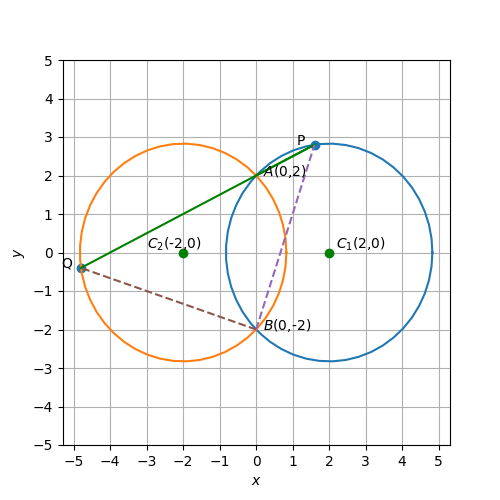
\includegraphics[width = \columnwidth]{chapters/9/10/6/9/figs/fig.png}
\caption{}
\label{fig:chapters/9/10/6/9/1}
\end{figure}

\item In any $\triangle ABC$, if the angle bisector of $\angle A$ and 
    perpendicular bisector of $BC$ intersect, prove that they intersect on 
    the circumcircle of $\triangle ABC$.
\\
    \solution 
\label{chapters/9/10/6/10}
\iffalse
\documentclass[journal,12pt,twocolumn]{IEEEtran}
\usepackage{setspace}
\usepackage{gensymb}
\singlespacing
\usepackage[cmex10]{amsmath}
\usepackage{amsthm}
\usepackage{mathrsfs}
\usepackage{txfonts}
\usepackage{stfloats}
\usepackage{bm}
\usepackage{cite}
\usepackage{cases}
\usepackage{subfig}
\usepackage{longtable}
\usepackage{multirow}
\usepackage{enumitem}
\usepackage{mathtools}
\usepackage{tikz}
\usepackage{circuitikz}
\usepackage{verbatim}
\usepackage[breaklinks=true]{hyperref}
\usepackage{tkz-euclide} % loads  TikZ and tkz-base
\usepackage{listings}
\usepackage{color}    
\usepackage{array}    
\usepackage{longtable}
\usepackage{calc}     
\usepackage{multirow} 
\usepackage{hhline}   
\usepackage{ifthen}   
\usepackage{lscape}     
\usepackage{chngcntr}
\DeclareMathOperator*{\Res}{Res}
\renewcommand\thesection{\arabic{section}}
\renewcommand\thesubsection{\thesection.\arabic{subsection}}
\renewcommand\thesubsubsection{\thesubsection.\arabic{subsubsection}}

\renewcommand\thesectiondis{\arabic{section}}
\renewcommand\thesubsectiondis{\thesectiondis.\arabic{subsection}}
\renewcommand\thesubsubsectiondis{\thesubsectiondis.\arabic{subsubsection}}
\renewcommand\thetable{\arabic{table}}
% correct bad hyphenation here
\hyphenation{op-tical net-works semi-conduc-tor}
\def\inputGnumericTable{}                                 %%

\lstset{
%language=C,
frame=single, 
breaklines=true,
columns=fullflexible
}
%\lstset{
%language=tex,
%frame=single, 
%breaklines=true
%}

\begin{document}
\newtheorem{theorem}{Theorem}[section]
\newtheorem{problem}{Problem}
\newtheorem{proposition}{Proposition}[section]
\newtheorem{lemma}{Lemma}[section]
\newtheorem{corollary}[theorem]{Corollary}
\newtheorem{example}{Example}[section]
\newtheorem{definition}[problem]{Definition}
\newcommand{\BEQA}{\begin{eqnarray}}
\newcommand{\EEQA}{\end{eqnarray}}
\newcommand{\define}{\stackrel{\triangle}{=}}
\bibliographystyle{IEEEtran}
\providecommand{\mbf}{\mathbf}
\providecommand{\pr}[1]{\ensuremath{\Pr\left(#1\right)}}
\providecommand{\qfunc}[1]{\ensuremath{Q\left(#1\right)}}
\providecommand{\sbrak}[1]{\ensuremath{{}\left[#1\right]}}
\providecommand{\lsbrak}[1]{\ensuremath{{}\left[#1\right.}}
\providecommand{\rsbrak}[1]{\ensuremath{{}\left.#1\right]}}
\providecommand{\brak}[1]{\ensuremath{\left(#1\right)}}
\providecommand{\lbrak}[1]{\ensuremath{\left(#1\right.}}
\providecommand{\rbrak}[1]{\ensuremath{\left.#1\right)}}
\providecommand{\cbrak}[1]{\ensuremath{\left\{#1\right\}}}
\providecommand{\lcbrak}[1]{\ensuremath{\left\{#1\right.}}
\providecommand{\rcbrak}[1]{\ensuremath{\left.#1\right\}}}
\theoremstyle{remark}
\newtheorem{rem}{Remark}
\newcommand{\sgn}{\mathop{\mathrm{sgn}}}
\providecommand{\abs}[1]{\left\vert#1\right\vert}
\providecommand{\res}[1]{\Res\displaylimits_{#1}} 
\providecommand{\norm}[1]{\left\lVert#1\right\rVert}
\providecommand{\mtx}[1]{\mathbf{#1}}
\providecommand{\mean}[1]{E\left[ #1 \right]}
\providecommand{\fourier}{\overset{\mathcal{F}}{ \rightleftharpoons}}
\providecommand{\system}[1]{\overset{\mathcal{#1}}{ \longleftrightarrow}}
\newcommand{\solution}{\noindent \textbf{Solution: }}
\newcommand{\cosec}{\,\text{cosec}\,}
\providecommand{\dec}[2]{\ensuremath{\overset{#1}{\underset{#2}{\gtrless}}}}
\newcommand{\myvec}[1]{\ensuremath{\begin{pmatrix}#1\end{pmatrix}}}
\newcommand{\mydet}[1]{\ensuremath{\begin{vmatrix}#1\end{vmatrix}}}
\let\vec\mathbf
\def\putbox#1#2#3{\makebox[0in][l]{\makebox[#1][l]{}\raisebox{\baselineskip}[0in][0in]{\raisebox{#2}[0in][0in]{#3}}}}
     \def\rightbox#1{\makebox[0in][r]{#1}}
     \def\centbox#1{\makebox[0in]{#1}}
     \def\topbox#1{\raisebox{-\baselineskip}[0in][0in]{#1}}
     \def\midbox#1{\raisebox{-0.5\baselineskip}[0in][0in]{#1}}

\vspace{3cm}
\title{Circle Assignment}
\author{Gautam Singh}
\maketitle
\bigskip

\begin{abstract}
    This document contains the solution to Question 10 of 
    Exercise 6 in Chapter 10 of the class 9 NCERT textbook.
\end{abstract}

\begin{enumerate}
    
    \fi
		Let the position vectors of the points be
    \begin{align}
        \vec{A} = \myvec{1\\0},\ \vec{B} = \myvec{\cos\beta\\\sin\beta},\ \vec{C} = \myvec{\cos\gamma\\\sin\gamma}
        \label{eq:chapters/9/10/6/10/pts}
    \end{align}

    Then, the equation of the perpendicular bisector of $BC$ is given by
    \begin{align}
        \norm{\vec{x}-\vec{B}}^2&=\norm{\vec{x}-\vec{C}}^2 \\
        \implies \brak{\vec{B}-\vec{C}}^\top\vec{x} &= 0
        \label{eq:chapters/9/10/6/10/perp-bisect}
    \end{align}
    and the equation of the angle bisector of $\angle A$ is given by
    \begin{align}
        &\frac{\brak{\vec{B}-\vec{A}}^\top\brak{\vec{x}-\vec{A}}}{\norm{\vec{B}-\vec{A}}} = \frac{\brak{\vec{C}-\vec{A}}^\top\brak{\vec{x}-\vec{A}}}{\norm{\vec{C}-\vec{A}}} \\
        &\brak{\frac{\vec{B}-\vec{A}}{\norm{\vec{B}-\vec{A}}}-\frac{\vec{C}-\vec{A}}{\norm{\vec{C}-\vec{A}}}}^\top\brak{\vec{x}-\vec{A}} = 0
        \label{eq:chapters/9/10/6/10/angle-bisect}
    \end{align}
    Note that from \eqref{eq:chapters/9/10/6/10/pts},
    \begin{align}
        \frac{\vec{B}-\vec{A}}{\norm{\vec{B}-\vec{A}}} &= \frac{1}{\sqrt{2\brak{1-\cos\beta}}}\myvec{\cos\beta-1\\\sin\beta} \\
                                                       &= \myvec{-\sin\frac{\beta}{2}\\\cos\frac{\beta}{2}}
                                                       \label{eq:chapters/9/10/6/10/unit-vec}
    \end{align}
    Therefore, using \eqref{eq:chapters/9/10/6/10/pts} in \eqref{eq:chapters/9/10/6/10/perp-bisect} and
    \eqref{eq:chapters/9/10/6/10/unit-vec} in \eqref{eq:chapters/9/10/6/10/angle-bisect},
    \begin{align}
        \myvec{\cos\beta-\cos\gamma\\\sin\beta-\sin\gamma}^\top\vec{x} &= 0 \label{eq:chapters/9/10/6/10/e1} \\
        \myvec{\sin\frac{\gamma}{2}-\sin\frac{\beta}{2}\\\cos\frac{\beta}{2}-\cos\frac{\gamma}{2}}^\top\vec{x} &= \sin\frac{\gamma}{2}-\sin\frac{\beta}{2} \label{eq:chapters/9/10/6/10/e2}
    \end{align}
    Using \eqref{eq:chapters/9/10/6/10/e1} and \eqref{eq:chapters/9/10/6/10/e2}, we form the matrix equation
    \begin{align}
        \myvec{\cos\beta-\cos\gamma&\sin\beta-\sin\gamma\\\sin\frac{\gamma}{2}-\sin\frac{\beta}{2}&\cos\frac{\beta}{2}-\cos\frac{\gamma}{2}}\vec{x} \nonumber \\
        = \myvec{0\\\sin\frac{\gamma}{2}-\sin\frac{\beta}{2}}
        \label{eq:chapters/9/10/6/10/mtx-eqn}
    \end{align}
    Solving \eqref{eq:chapters/9/10/6/10/mtx-eqn} using the augmented matrix, and letting 
    $\theta \triangleq \frac{\beta+\gamma}{2}$,
    \begin{align}
        &\myvec{\cos\beta-\cos\gamma&\sin\beta-\sin\gamma&0\\\sin\frac{\gamma}{2}-\sin\frac{\beta}{2}&\cos\frac{\beta}{2}-\cos\frac{\gamma}{2}&\sin\frac{\gamma}{2}-\sin\frac{\beta}{2}} \\
        &\xleftrightarrow[]{\substack{R_1\leftarrow\frac{R_1}{\cos\beta-\cos\gamma}\\R_2\leftarrow\frac{R_2}{\sin\frac{\gamma}{2}-\sin\frac{\beta}{2}}}}\myvec{1&-\cot\theta&0\\1&\tan\frac{\theta}{2}&1} \\
        &\xleftrightarrow[]{R_2\leftarrow R_2-R_1}\myvec{1&-\cot\theta&0\\0&\tan\frac{\theta}{2}+\cot\theta&1} \\
        &= \myvec{1&-\cot\theta&0\\0&\csc\theta&1} \\
        &\xleftrightarrow[]{R_1\leftarrow R_1 + R_2\cos\theta}\myvec{1&0&\cos\theta\\0&\csc\theta&1} \\
        &\xleftrightarrow[]{R_2\leftarrow R_2\sin\theta}\myvec{1&0&\cos\theta\\0&1&\sin\theta}
        \label{eq:chapters/9/10/6/10/aug-mtx}
    \end{align}
    Thus, the intersection of the lines in \eqref{eq:chapters/9/10/6/10/e1} and \eqref{eq:chapters/9/10/6/10/e2} is
    \begin{align}
        \vec{D} \triangleq \myvec{\cos\frac{\beta+\gamma}{2}\\\sin\frac{\beta+\gamma}{2}}
        \label{eq:chapters/9/10/6/10/intersect-pt}
    \end{align}
    Hence, it is clear from \eqref{eq:chapters/9/10/6/10/intersect-pt} that $\vec{D}$ lies on the 
    circumcircle of $\triangle ABC$, as required.

    The situation is illustrated in Fig. \ref{fig:chapters/9/10/6/10/bisector}. The parameters
    used in the construction are shown in Table \ref{tab:chapters/9/10/6/10/param}.
    \begin{table}[!ht]
        \centering
        %%%%%%%%%%%%%%%%%%%%%%%%%%%%%%%%%%%%%%%%%%%%%%%%%%%%%%%%%%%%%%%%%%%%%%
%%                                                                  %%
%%  This is the header of a LaTeX2e file exported from Gnumeric.    %%
%%                                                                  %%
%%  This file can be compiled as it stands or included in another   %%
%%  LaTeX document. The table is based on the longtable package so  %%
%%  the longtable options (headers, footers...) can be set in the   %%
%%  preamble section below (see PRAMBLE).                           %%
%%                                                                  %%
%%  To include the file in another, the following two lines must be %%
%%  in the including file:                                          %%
%%        \def\inputGnumericTable{}                                 %%
%%  at the beginning of the file and:                               %%
%%        \input{name-of-this-file.tex}                             %%
%%  where the table is to be placed. Note also that the including   %%
%%  file must use the following packages for the table to be        %%
%%  rendered correctly:                                             %%
%%    \usepackage[latin1]{inputenc}                                 %%
%%    \usepackage{color}                                            %%
%%    \usepackage{array}                                            %%
%%    \usepackage{longtable}                                        %%
%%    \usepackage{calc}                                             %%
%%    \usepackage{multirow}                                         %%
%%    \usepackage{hhline}                                           %%
%%    \usepackage{ifthen}                                           %%
%%  optionally (for landscape tables embedded in another document): %%
%%    \usepackage{lscape}                                           %%
%%                                                                  %%
%%%%%%%%%%%%%%%%%%%%%%%%%%%%%%%%%%%%%%%%%%%%%%%%%%%%%%%%%%%%%%%%%%%%%%



%%  This section checks if we are begin input into another file or  %%
%%  the file will be compiled alone. First use a macro taken from   %%
%%  the TeXbook ex 7.7 (suggestion of Han-Wen Nienhuys).            %%
\def\ifundefined#1{\expandafter\ifx\csname#1\endcsname\relax}


%%  Check for the \def token for inputed files. If it is not        %%
%%  defined, the file will be processed as a standalone and the     %%
%%  preamble will be used.                                          %%
\ifundefined{inputGnumericTable}

%%  We must be able to close or not the document at the end.        %%
	\def\gnumericTableEnd{\end{document}}


%%%%%%%%%%%%%%%%%%%%%%%%%%%%%%%%%%%%%%%%%%%%%%%%%%%%%%%%%%%%%%%%%%%%%%
%%                                                                  %%
%%  This is the PREAMBLE. Change these values to get the right      %%
%%  paper size and other niceties.                                  %%
%%                                                                  %%
%%%%%%%%%%%%%%%%%%%%%%%%%%%%%%%%%%%%%%%%%%%%%%%%%%%%%%%%%%%%%%%%%%%%%%

	\documentclass[12pt%
			  %,landscape%
                    ]{report}
       \usepackage[latin1]{inputenc}
       \usepackage{fullpage}
       \usepackage{color}
       \usepackage{array}
       \usepackage{longtable}
       \usepackage{calc}
       \usepackage{multirow}
       \usepackage{hhline}
       \usepackage{ifthen}

	\begin{document}


%%  End of the preamble for the standalone. The next section is for %%
%%  documents which are included into other LaTeX2e files.          %%
\else

%%  We are not a stand alone document. For a regular table, we will %%
%%  have no preamble and only define the closing to mean nothing.   %%
    \def\gnumericTableEnd{}

%%  If we want landscape mode in an embedded document, comment out  %%
%%  the line above and uncomment the two below. The table will      %%
%%  begin on a new page and run in landscape mode.                  %%
%       \def\gnumericTableEnd{\end{landscape}}
%       \begin{landscape}


%%  End of the else clause for this file being \input.              %%
\fi

%%%%%%%%%%%%%%%%%%%%%%%%%%%%%%%%%%%%%%%%%%%%%%%%%%%%%%%%%%%%%%%%%%%%%%
%%                                                                  %%
%%  The rest is the gnumeric table, except for the closing          %%
%%  statement. Changes below will alter the table's appearance.     %%
%%                                                                  %%
%%%%%%%%%%%%%%%%%%%%%%%%%%%%%%%%%%%%%%%%%%%%%%%%%%%%%%%%%%%%%%%%%%%%%%

\providecommand{\gnumericmathit}[1]{#1} 
%%  Uncomment the next line if you would like your numbers to be in %%
%%  italics if they are italizised in the gnumeric table.           %%
%\renewcommand{\gnumericmathit}[1]{\mathit{#1}}
\providecommand{\gnumericPB}[1]%
{\let\gnumericTemp=\\#1\let\\=\gnumericTemp\hspace{0pt}}
 \ifundefined{gnumericTableWidthDefined}
        \newlength{\gnumericTableWidth}
        \newlength{\gnumericTableWidthComplete}
        \newlength{\gnumericMultiRowLength}
        \global\def\gnumericTableWidthDefined{}
 \fi
%% The following setting protects this code from babel shorthands.  %%
 \ifthenelse{\isundefined{\languageshorthands}}{}{\languageshorthands{english}}
%%  The default table format retains the relative column widths of  %%
%%  gnumeric. They can easily be changed to c, r or l. In that case %%
%%  you may want to comment out the next line and uncomment the one %%
%%  thereafter                                                      %%
\providecommand\gnumbox{\makebox[0pt]}
%%\providecommand\gnumbox[1][]{\makebox}

%% to adjust positions in multirow situations                       %%
\setlength{\bigstrutjot}{\jot}
\setlength{\extrarowheight}{\doublerulesep}

%%  The \setlongtables command keeps column widths the same across  %%
%%  pages. Simply comment out next line for varying column widths.  %%
\setlongtables

\setlength\gnumericTableWidth{%
	60pt+%
	67pt+%
0pt}
\def\gumericNumCols{2}
\setlength\gnumericTableWidthComplete{\gnumericTableWidth+%
         \tabcolsep*\gumericNumCols*2+\arrayrulewidth*\gumericNumCols}
\ifthenelse{\lengthtest{\gnumericTableWidthComplete > \linewidth}}%
         {\def\gnumericScale{1*\ratio{\linewidth-%
                        \tabcolsep*\gumericNumCols*2-%
                        \arrayrulewidth*\gumericNumCols}%
{\gnumericTableWidth}}}%
{\def\gnumericScale{1}}

%%%%%%%%%%%%%%%%%%%%%%%%%%%%%%%%%%%%%%%%%%%%%%%%%%%%%%%%%%%%%%%%%%%%%%
%%                                                                  %%
%% The following are the widths of the various columns. We are      %%
%% defining them here because then they are easier to change.       %%
%% Depending on the cell formats we may use them more than once.    %%
%%                                                                  %%
%%%%%%%%%%%%%%%%%%%%%%%%%%%%%%%%%%%%%%%%%%%%%%%%%%%%%%%%%%%%%%%%%%%%%%

\ifthenelse{\isundefined{\gnumericColA}}{\newlength{\gnumericColA}}{}\settowidth{\gnumericColA}{\begin{tabular}{@{}p{60pt*\gnumericScale}@{}}x\end{tabular}}
\ifthenelse{\isundefined{\gnumericColB}}{\newlength{\gnumericColB}}{}\settowidth{\gnumericColB}{\begin{tabular}{@{}p{67pt*\gnumericScale}@{}}x\end{tabular}}

\begin{tabular}[c]{%
	b{\gnumericColA}%
	b{\gnumericColB}%
	}

%%%%%%%%%%%%%%%%%%%%%%%%%%%%%%%%%%%%%%%%%%%%%%%%%%%%%%%%%%%%%%%%%%%%%%
%%  The longtable options. (Caption, headers... see Goosens, p.124) %%
%	\caption{The Table Caption.}             \\	%
% \hline	% Across the top of the table.
%%  The rest of these options are table rows which are placed on    %%
%%  the first, last or every page. Use \multicolumn if you want.    %%

%%  Header for the first page.                                      %%
%	\multicolumn{2}{c}{The First Header} \\ \hline 
%	\multicolumn{1}{c}{colTag}	%Column 1
%	&\multicolumn{1}{c}{colTag}	\\ \hline %Last column
%	\endfirsthead

%%  The running header definition.                                  %%
%	\hline
%	\multicolumn{2}{l}{\ldots\small\slshape continued} \\ \hline
%	\multicolumn{1}{c}{colTag}	%Column 1
%	&\multicolumn{1}{c}{colTag}	\\ \hline %Last column
%	\endhead

%%  The running footer definition.                                  %%
%	\hline
%	\multicolumn{2}{r}{\small\slshape continued\ldots} \\
%	\endfoot

%%  The ending footer definition.                                   %%
%	\multicolumn{2}{c}{That's all folks} \\ \hline 
%	\endlastfoot
%%%%%%%%%%%%%%%%%%%%%%%%%%%%%%%%%%%%%%%%%%%%%%%%%%%%%%%%%%%%%%%%%%%%%%

\hhline{|-|-}
	 \multicolumn{1}{|p{\gnumericColA}|}%
	{\gnumericPB{\centering}\gnumbox{\textbf{Parameter}}}
	&\multicolumn{1}{p{\gnumericColB}|}%
	{\gnumericPB{\centering}\gnumbox{\textbf{Value}}}
\\
\hhline{|--|}
	 \multicolumn{1}{|p{\gnumericColA}|}%
	{\gnumericPB{\centering}\gnumbox{$r$}}
	&\multicolumn{1}{p{\gnumericColB}|}%
	{\gnumericPB{\centering}\gnumbox{1}}
\\
\hhline{|--|}
	 \multicolumn{1}{|p{\gnumericColA}|}%
	{\gnumericPB{\centering}\gnumbox{$\beta$}}
	&\multicolumn{1}{p{\gnumericColB}|}%
    {\gnumericPB{\centering}\gnumbox{100$^{\circ}$}}
\\
\hhline{|--|}
	 \multicolumn{1}{|p{\gnumericColA}|}%
	{\gnumericPB{\centering}\gnumbox{$\gamma$}}
	&\multicolumn{1}{p{\gnumericColB}|}%
    {\gnumericPB{\centering}\gnumbox{200$^{\circ}$}}
\\
\hhline{|-|-|}
\end{tabular}

\ifthenelse{\isundefined{\languageshorthands}}{}{\languageshorthands{\languagename}}
\gnumericTableEnd

        \caption{Parameters used in the construction of Fig. \ref{fig:chapters/9/10/6/10/bisector}.}
        \label{tab:chapters/9/10/6/10/param}
    \end{table}
    \begin{figure}[!ht]
        \centering
        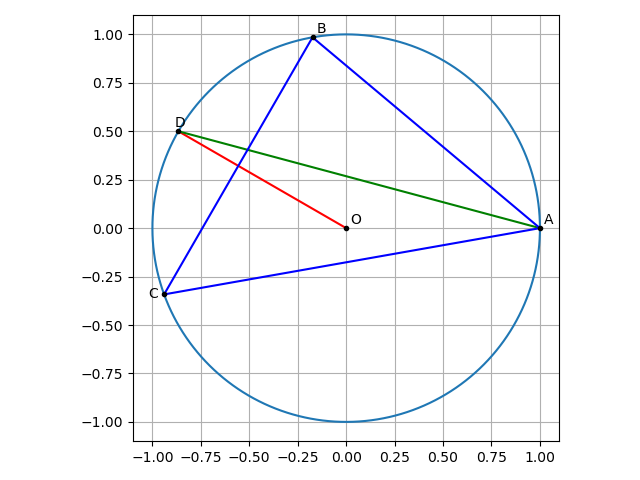
\includegraphics[width=\columnwidth]{chapters/9/10/6/10/figs/bisector.png}
        \caption{The bisector of $\angle A$ and of $BC$ meet on the circumcircle at $D$.}
        \label{fig:chapters/9/10/6/10/bisector}
    \end{figure}


\end{enumerate}
